% Section content template for individual Educative lessons
% This file contains the actual content for a specific section
% Generated from Educative API section content

% Section: Requirements for the Chess Game
% Section ID: 5244835679436800
% Section Slug: requirements-for-the-chess-game
% Generated: 2025-12-12T16:10:31.291301

This lesson outlines the functional and operational requirements for an online chess game. Identifying and understanding requirements is essential to defining the system's scope and ensuring a robust, user-friendly design.
\\
We'll use the notational convention to identify each requirement with a unique label ``Rn,'' where ``R'' is short for requirement and ``n'' is a natural number.

\subsection{Requirement collection}\label{kClQrdblfqCg5z07HsqrP}

% \vspace{-1.0\baselineskip}
\noindent
\begin{minipage}[t]{0.48\textwidth}\vspace{0pt}
\begin{itemize}
\item
\textbf{R1:} The system must enable two players (human or machine) to play chess online, supporting real-time, turn-based multiplayer gameplay.
\item
\textbf{R2:} The chess game must strictly enforce the official rules of international (standard) chess.
\end{itemize}
\end{minipage}
\hfill
\begin{minipage}[t]{0.48\textwidth}\vspace{0pt}
\centering
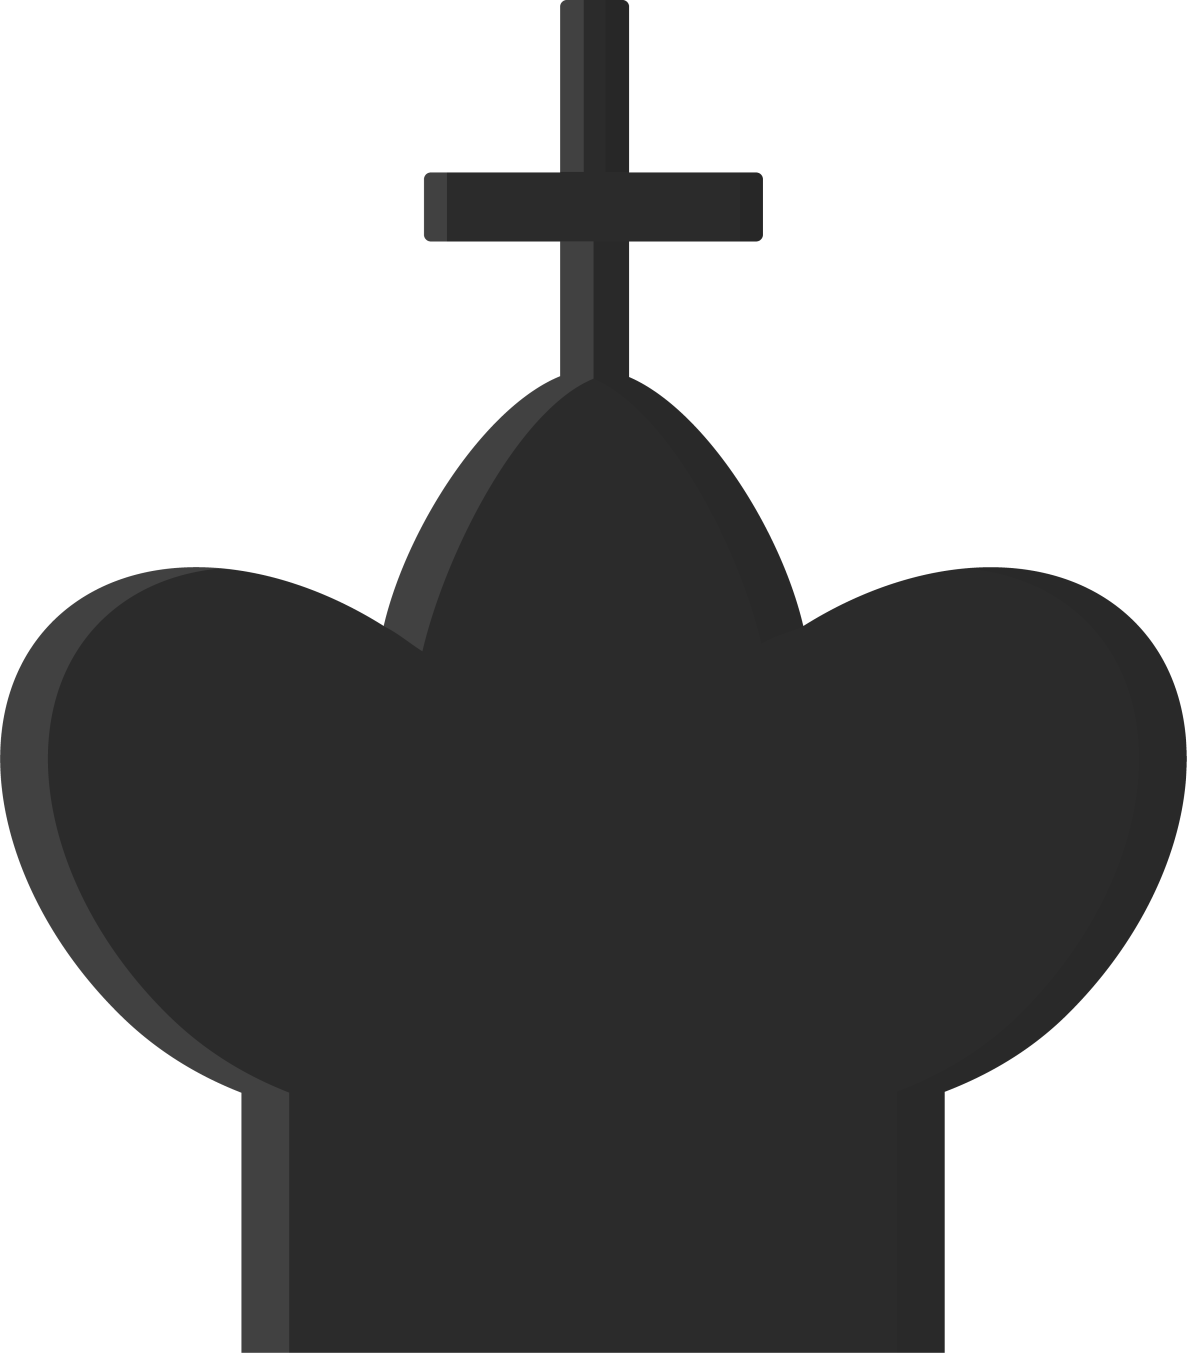
\includegraphics[width=0.5\textwidth]{Images/chapter_17/section_5244835679436800/5415473643782144.png}
\end{minipage}

% \vspace{-1.0\baselineskip}
\noindent
\begin{minipage}[t]{0.48\textwidth}\vspace{0pt}
\begin{itemize}
\item
\textbf{R3:} At the beginning of each game, players will be randomly assigned white or black.
\item
\textbf{R4:} Each player starts with 16 pieces: eight pawns, two rooks, two knights, two bishops, one queen, and one king, placed in the official starting positions on the 8x8 chessboard.
\end{itemize}
\end{minipage}
\hfill
\begin{minipage}[t]{0.48\textwidth}\vspace{0pt}
\centering

\includegraphics[width=0.5\textwidth]{Images/chapter_17/section_5244835679436800/4668715934416896.png}
\end{minipage}

% \vspace{-1.0\baselineskip}
\noindent
\begin{minipage}[t]{0.48\textwidth}\vspace{0pt}
\begin{itemize}
\item
\textbf{R5:} The player with the white pieces always makes the first move.
\item
\textbf{R6:} Players may not retract or undo their moves once made. (No ``take-back'' or undo functionality.)
\end{itemize}
\end{minipage}
\hfill
\begin{minipage}[t]{0.48\textwidth}\vspace{0pt}
\centering

\includegraphics[width=0.5\textwidth]{Images/chapter_17/section_5244835679436800/6106052946034688.png}
\end{minipage}

% \vspace{-1.0\baselineskip}
\noindent
\begin{minipage}[t]{0.48\textwidth}\vspace{0pt}
\begin{itemize}
\item
\textbf{R8:}~The game must support all official ways a chess game can end, including:

\begin{itemize}
\item
Checkmate (a player's king is under attack and cannot escape)
\item
Stalemate (no legal moves, and the king is not in check)
\item
Draw (mutual agreement, threefold repetition, 50-move rule, or insufficient material)
\item
Resignation (a player concedes defeat)
\item
Forfeiture (a player does not show up or abandons the game)
\end{itemize}
\item
\textbf{R9:} According to international chess rules, the system must support special moves such as castling, en passant, and pawn promotion.
\end{itemize}
\end{minipage}
\hfill
\begin{minipage}[t]{0.48\textwidth}\vspace{0pt}
\centering

\includegraphics[width=0.5\textwidth]{Images/chapter_17/section_5244835679436800/6070964673839104.png}
\end{minipage}

\begin{figure}[htbp]
 \centering
 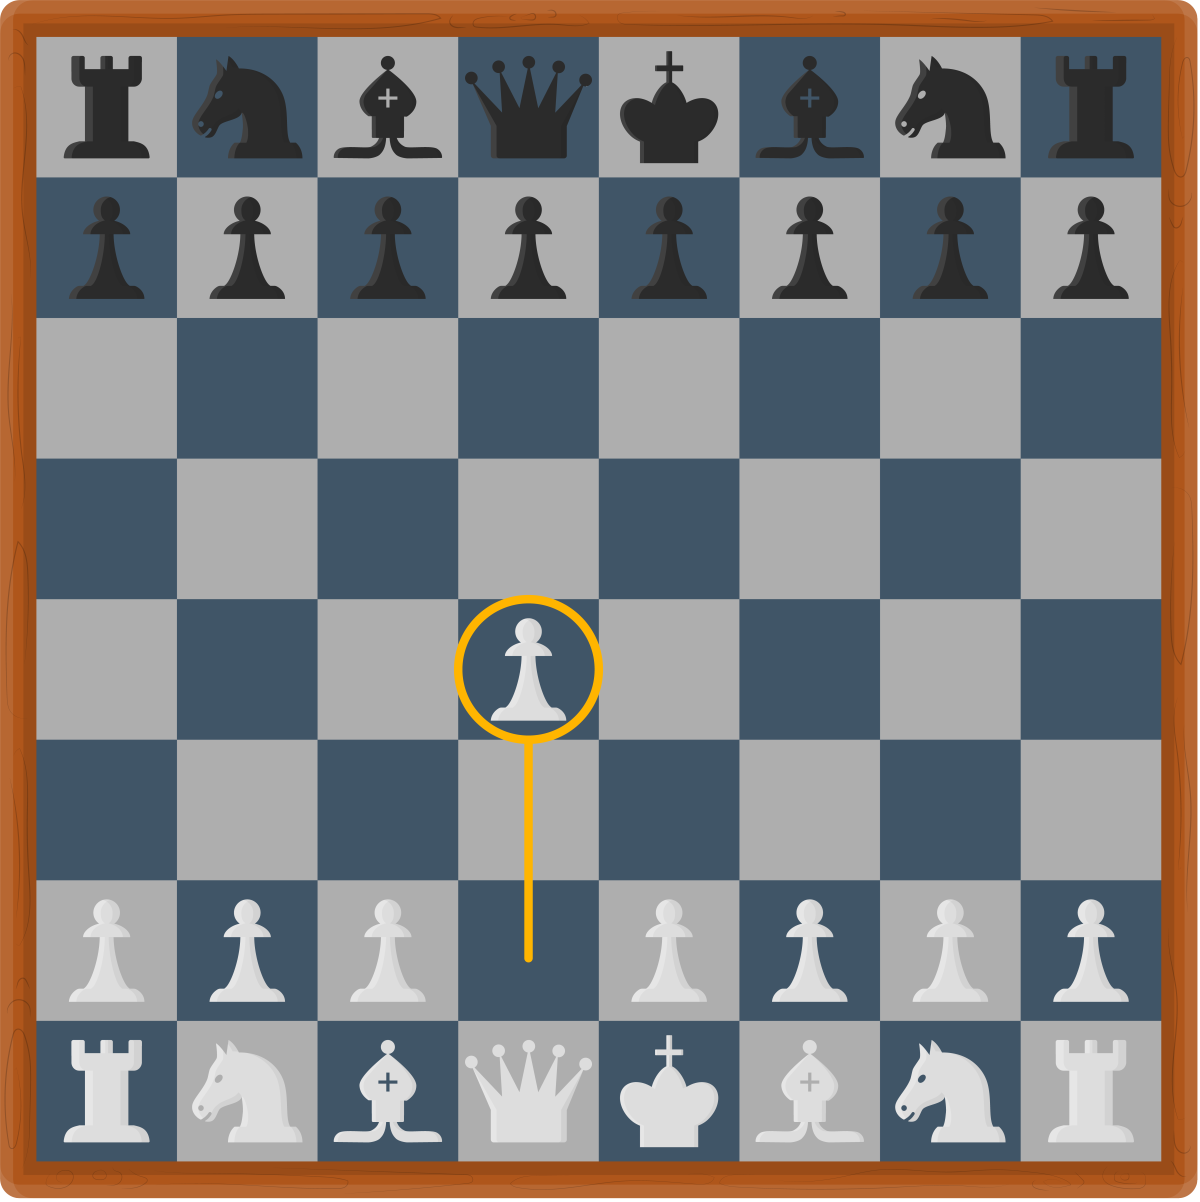
\includegraphics[width=0.5\textwidth]{Images/chapter_17/section_5244835679436800/5389002451714048.png}
 \caption{White pawn takes the first move}
\end{figure}

\subsection{International chess rules}\label{PKUZU5MGk9g6Kne4r0CFv}

\subsubsection{Rules for pieces}\label{hVPJ6gsUFgUEKtg84G-7C}
\\
The following table represents the basic rules of chess:

\begin{table}[h!]
\centering
\begin{tabular}{|p{3cm}|p{12cm}|}
\hline
\textbf{Piece} & \textbf{Movement Rules} \\
\hline
King & 
Moves one square in any direction (horizontally, vertically, or diagonally).
May perform castling once per game with a rook, if neither piece has moved,
no pieces are between them, and the king does not move through, into,
or out of check. \\
\hline
Queen & 
Moves any number of squares vertically, horizontally, or diagonally.
Cannot jump over other pieces. \\
\hline
Rook & 
Moves any number of squares vertically or horizontally.
Cannot jump over other pieces.
Participates in castling with the king. \\
\hline
Bishop & 
Moves any number of squares diagonally.
Cannot jump over other pieces. \\
\hline
Knight & 
Moves in an ``L-shape'': two squares in one direction (horizontal or vertical),
then one square perpendicular.
Can jump over other pieces. \\
\hline
Pawn & 
Moves forward one square.
On its first move, it may move forward two squares.
Captures one square diagonally forward.
Can perform en passant capture.
Promotes to queen, rook, bishop, or knight upon reaching the last rank. \\
\hline
\end{tabular}
\caption{Chess Pieces and Their Movement Rules}
\label{tab:chess_movement_rules}
\end{table}


\subsubsection{Rules for situations}\label{KZamHAF28JI3gYS4kZE55}
\\
The following table represents certain situations we might face while playing chess:

\begin{table}[h!]
\centering
\begin{tabular}{|p{3.5cm}|p{11.5cm}|}
\hline
\textbf{Situation} & \textbf{Description / Rule} \\
\hline
Check &
The king is under threat of capture.
The player must make a move to remove the check. \\
\hline
Checkmate &
The king is in check and has no legal moves to escape.
The game ends, and the opponent wins. \\
\hline
Stalemate &
The player has no legal moves, and their king is not in check.
The game ends in a draw. \\
\hline
Draw &
Can occur due to stalemate, threefold repetition, the 50-move rule
(50 moves by each player with no pawn move or capture), insufficient material,
or mutual agreement. \\
\hline
Forfeiture &
A player forfeits if they do not show up for the game or abandon it. \\
\hline
Resignation &
A player may resign at any time, conceding the game to the opponent. \\
\hline
Castling &
A special move involving the king and a rook, performed on either the
kingside or queenside. Allowed only if:
\begin{itemize}
    \item Neither the king nor the chosen rook has moved.
    \item There are no pieces between the king and the rook.
    \item The king is not in check, does not move through a square under attack,
          and does not end up in check.
    \item The king has not previously been in check.
\end{itemize}
The king moves two squares toward the rook, and the rook moves to the square
the king passed over. \\
\hline
En Passant &
A pawn that advances two squares from its starting position may be captured
``en passant'' by an opposing pawn as if it had moved only one square.
This capture must be made immediately on the next move. \\
\hline
Pawn Promotion &
When a pawn reaches the farthest rank from its starting position, it is promoted
to a queen, rook, bishop, or knight, as chosen by the player. \\
\hline
\end{tabular}
\caption{Special Situations and Rules in Chess}
\label{tab:chess_special_rules}
\end{table}


We've identified our requirements for the problem. The next lesson will define different use cases for the online chess game design.

% End of section content